\chapter{Implementation}

\begin{figure}[h]
\centering
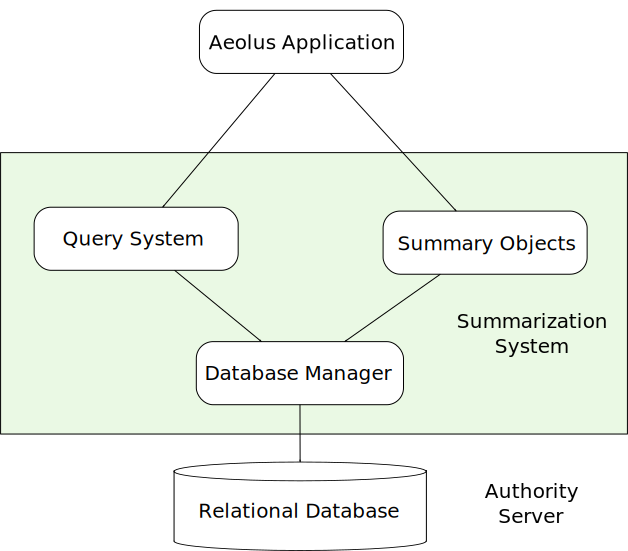
\includegraphics[width=.8\textwidth,keepaspectratio]{figures/impl-sysarch}
\caption[Summarization System Architecture]{Summarization System Architecture. This diagram illustrates the components involved in the summarization system we provide.}
\label{fig:impl-sysarch}
\end{figure}

The codebase for this thesis is implemented in approximately 4000 lines of Java code, of which 3000 implement the Mint application and 1000 implement the summarization system. The focus of this chapter is the implementation of the summarization system.

Figure \ref{fig:impl-sysarch} presents a high-level overview of the summarization system components. The application uses the Query System (QS) and Summary Objects (SOs) to produce summaries and mark events. The Database Manager (DBM) stores queries and summaries in a PostgreSQL relational database \cite{pgsql-gen}, as well as retrieves results of queries. On VN startup, we create the extra QUERY, SUMMARY, LOG-MARKED and SUMMARY-MARKED tables necessary for the running of the summarization system.

The rest of this chapter describes the implementation of those components.

\section{The Query System and The Summary Objects}

The QS provides the interface described in section \ref{model:query-system} and a Summary Object provides the interface described in section \ref{model:summary-objects}. Summary Objects store the name and parameters of the underlying query locally.

Both the QS and the SOs are responsible for logging calls to their methods as described in sections \ref{model:query-system} and \ref{model:summary-objects}.

\section{The Database Manager}

All communications to the relational database go through the DBM. The DBM provides an internal interface for the QS and SOs to carry out the various operations necessary.

\begin{description}
  \item[setUpSummarizationSystem()] \ \\
    This method creates the 

    This method is called by the QS.
  \item[\emph{addQuery(name, query\_text)}] \ \\
    Executes a SQL INSERT statement to add a record
    to the QUERY table with the values \emph{name}
    and \emph{query\_text}.
    Throws an exception if the labels of the 
    calling thread are not empty.

    This method is called by the QS.
  \item[\emph{runQuery(name, vals)}] \ \\
    This call carries out the following actions,
    in order:
    \begin{enumerate}
      \item Executes a SQL SELECT statement to retrieve 
        the query text from the QUERY table.
      \item Uses a Java PreparedStatement to combine
        the query text with the values in the 
        \emph{vals} array,
        and throws an exception if the expected
        number or type of parameters do not match
        the ones provided.
      \item Modifies the query to exclude any marked events.
        For example, if the combined query text was 
        \begin{lstlisting}[language=SQL]
        select * from events where 
        app_opp='mint-user-signup'
        \end{lstlisting}
        the DBM modifies it to the following
        \begin{lstlisting}[language=SQL]
        select * from (select * 
        from events where app_op='mint-user-signup') 
        as e where e.event_counter not in 
        (select event_counter from events-marked)
        \end{lstlisting}
        We use a subquery to carry out the task to avoid
        having to parse the query for a an already-existing
        \lstinline$where$ clause in the query.
      \item Executes the combined query text and
        retrieves the set of records covered by that query.
      \item Removes from the retrieved set of records
        any records that
        the calling thread is not allowed
        to view per the DIFC rules described in section
        \ref{difc:rules}, then returns the resulting
        set of records.
    \end{enumerate}
    This method is called by the QS and the SO constructor.
  \item[\emph{addSummary(s\_name, 
      s\_args, q\_name, q\_ args, tstamp)}] \ \\
    \emph{s\_name} is the summary name, \emph{q\_name}
    is the query name (similarly for \emph{s\_args} and
    \emph{q\_args}. \emph{tstamp} is the timestamp.
    Executes a SQL INSERT statement to add a record to
    the SUMMARY table, using the arguments and labels
    of the calling thread as as values for the record.
    
    This method is called by the SOs.
  \item[\emph{mark(query\_name, query\_params)}] \ \\
    Executes a SQL INSERT statement to add events
    to the LOG-MARKED and SUMMARY-MARKED tables to
    identify marked records.
    Event counters in the SUMMARY table contain
    a non-numeric character to distinguish them from
    event counters in the LOG. The DBM uses 
    this knowledge to distinguish
    where to add a marked event (LOG-MARKED or 
    SUMMARY-MARKED).
    
    This method is called by the SOs.
\end{description}

In an ideal implementation, our system would be using the PostgreSQL Information Flow Control database provided by David Schultz \cite{das}. This would push the tasks of enforcing empty labels when adding queries and filtering query results according to the label of the calling thread to the database itself to handle.

\subsection{Running in \emph{Hide} Mode}

Once events are marked, they are hidden from the application in future queries. This is implemented by introducing a two views, LOG-UNMARKED and SUMMARY-UNMARKED, that only contains events that are in the LOG and SUMMARY tables but not in the LOG-MARKED and SUMMARY-MARKED tables. We expose only the names of the LOG-UNMARKED and SUMMARY-UNMARKED views to the application for writing queries.

Our system can be extended to implement a \emph{no-hide} mode, where the LOG-UNMARKED and SUMMARY-UNMARKED views show exactly the same records as the LOG and the SUMMARY tables.
